\documentclass[12pt,a4paper]{article}
\usepackage{amsmath,amssymb,graphicx}
\usepackage{bbm}
\usepackage{authblk}
\usepackage{faktor}
\usepackage{caption}
\usepackage{subcaption}
\usepackage{float}
% \usepackage{tcolorbox}
\usepackage[utf8]{inputenc}
\usepackage[english]{babel}
\usepackage{listings}
\usepackage{color}


\begin{document}

\title{ Notes on Simple Nets }

\author[$\dagger$]{}
%\affil[$\dagger$]{Department of Theoretical Physics, Maynooth University}
\date{}

\maketitle


\section{Overall plan}

(v.1: Masud, August 2019)

The current idea of the project:

\begin{center}\emph{Fitness landscape of 3-node and 4-node neural networks}
\end{center}

Restricting to one input node and one output node, we can think of three network geometries:

\begin{center}
\begin{tabular}{l|l}
\hline
%
\parbox{0.42\textwidth}{ 
%

\begin{center}\includegraphics[width=0.4\textwidth]{Images/3_architectures_a_01}
\end{center}


} &   \hspace{-0.01\textwidth}
\parbox{0.48\textwidth}{ \flushleft

\begin{itemize}

\item[(A)] One hidden layer, containing a single hidden node. \\ 4 parameters. 

\bigskip 

\item[(B)] Two hidden layers, each containing a single node. 
  \\ 6 parameters.
  
\bigskip 

\item[(C)] One hidden layer, consisting of two nodes. 
  \\ 7 parameters.
  
\end{itemize}

} 
\\
\hline
\end{tabular}
\end{center}



We can then explore and describe the landscape of the loss function for the same (or similar)
learning task in these three cases.  In addition, we can explore and describe how the gradient descent moves us along
this landscape.

The three networks have respectively 4, 6 and 7 parameters.

The primary learning task with these networks will be to learn a scalar function.  The function
$f(x) = x^2$ seems the most natural to concentrate on.  We still have to specify the domain of the
function (interval from which $x$ is chosen) over which to concentrate on.  We might want to use the
sigmoid function in the definition of the network; in that case the outputs are limited to $[0,1]$.
Hence it makes sense to use the interval $[-1,1]$.

The 3-node network (A) is so limited that it is not able to approximate the parabolic shape in the
whole range $[-1,1]$ (please double-check this statement), so we will probably have to limit it to
$[0,1]$.

The choice of activation function defines the network, i.e., the loss function will depend on the
activation function.  Let's start with the sigmoid whenever we can, and possibly play with using
other activation functions later.


\subsection{The functions expressed by the toy networks} 


For the 3-node network A, the output as a function of the input $x$ is
\begin{equation} \label{eq_intro_3node_function}
[A]  \qquad \qquad N(x) ~=~  \sigma\Big( w^2_{11} \sigma\big(w^1_{11}x+b^1_1\big) +b^2_1 \Big)
\end{equation}
where the superscript/subscript notation is that of Nielsen, see, e.g., the diagram in
%
\\ {\tt http://neuralnetworksanddeeplearning.com/chap2.html}
%
\\ The same notation is probably standard elsewhere as well.  The superscripts are layer indices and
the in the subscript $ij$ for the $w$'s, the first is an index for the nodes of the previous layer
and the second is the index for the nodes of the current layer.  (The input layer is called layer 0
here.)  This elaborate notation is probably overkill for the toy networks we will be using; we will
use simpler names later on when we focus on the individual networks.

The problem of learning the $x^2$ function with the network A is simply the problem of
least-square-fitting the above nonlinear function to a dataset of the form $\{(u,u^2)\}$. 

Similarly, the functions expressed by the other two networks are 
\begin{equation} 
[B]  \qquad \qquad N(x) ~=~   \sigma\Bigg( w^3_{11} \sigma\Big( w^2_{11} \sigma\big(w^1_{11}x+b^1_1\big) +b^2_1 \Big) +b^3_1 \Bigg)
\end{equation}
and 
\begin{equation} 
  [C]  \qquad \qquad
N(x) ~=~  \sigma\Big( w^2_{11} \sigma\big(w^1_{11}x+b^1_1\big) + w^2_{21} \sigma\big(w^1_{12}x+b^1_2\big) +b^2_1 \Big)  
\end{equation}
%
We should probably use simpler notations while discussing the individual networks.  


\subsection{Choice of activation function}

Should we choose activation functions that are well-suited for learning  the $x^2$ function, or
choose those that are bad for the present purpose?  The suitability of the activation function
probably affects the nature of the fitness landscape, so both might be interesting.  However, let's
start with choosing activation functions that allow us to do a relatively good job.  

Given the nature of the problem --- fitting a nonlinear (quadratic) function --- a piecewise linear
function will probably not do a good job.  (Maybe we should check this statement.)  This rules out
the RelU function.

So let's concentrate on the sigmoid function
\[
\sigma(x) ~=~ \frac{1}{1+e^{-x}}
\]
and the softplus function
\[
\sigma(x) ~=~ \log(1 + e^x)
\]
The softplus is a rounded version of the RelU.  



\newpage 


\section{The 3-node network}

(v.1: Masud, August 2019)

\subsection{Setup}



\begin{center}
\begin{tabular}{l|l}
%\hline
%
\parbox{0.48\textwidth}{ 
%
\raggedright
  
Let's simplify the notation; one index should suffice.  The four parameters are $w_1$ and $b_1$
(determining the hidden-neuron value from the input value $x$) and $w_2$ and $b_2$ (which determine the
final output from the hidden-neuron value).
  


} &   \hspace{-0.01\textwidth}
\parbox{0.42\textwidth}{ \flushleft


\begin{center}
\includegraphics[width=0.35\textwidth]{Images/notation_3node_a_01}
\end{center}

\begin{gather*}
  z_1 = w_1x + b_1
  \\
  z_2 = w_2\sigma(z_1) + b_2
  \\
  {\rm output} = \sigma(z_2)
\end{gather*}


} 
\\
%\hline
\end{tabular}
\end{center}



The function represented by the network is
\begin{equation}
N(x) ~=~  \sigma\Big( w_2 \sigma\big(w_1x+b_1\big) +b_2 \Big)
\end{equation}
So the quantity we want to analyze is
\begin{equation}
L(w_1,w_2,b_1,b_2) ~=~  \int_{x_{\rm min}}^{x_{\rm max}} \Big[ N(x) -x^2 \Big]^2 
\end{equation}
In practice we want to discretize this integral and have a sum over a grid of $x$ values.  Hopefully
the answer does not depend much on the discretization.  

Define
\[
x_i = x_{\rm min} + \frac{x_{\rm max} - x_{\rm min}}{n_T} i
\qquad \qquad  \text{with} \quad i = 0, 1,\ldots, n_T
\]
The subscript $T$ could stand for `test', as the set of numbers $\{(x_i,x_i^2)\}$ can be regarded as
the test set used to define the fitness function or loss function.  However, for the present
toy problem, there is probably no harm to use the same set as the training set.

The loss/fitness function we aim to analyze is thus 
\begin{equation}
L(w_1,w_2,b_1,b_2) ~=~  \frac{x_{\rm max} - x_{\rm min}}{n_T} \sum_{i=0}^{n_T} \Big[ N(x_i) -x_i^2 \Big]^2 
\end{equation}
%
We expect that the results should not depend on $n_T$ as long as it is `large enough'; perhaps
even $n_T=20$ is large enough. 

If some other target function $f(x)$ is being trained for instead of $f(x)=x^2$, one simply replaces
$x_i^2$ by $f(x_i)$ in the above expression.  


\subsection{Some observations }

Played with minimizing the loss function using the minimizers provided by Mathematica.  (The
FindMinimum[] function.)

The performance of this primitive network as a learner/predictor is rather limited --- it seems not
able to fit even roughly the $x^2$ function in the range (-1,1).  Using the sigmoid function, it
even has difficulty fitting in the range (0,1).  The  Softplus function does a better job.

The landscape seems interesting enough --- there are multiple minima for sure.  It also parameter
regimes in which the loss function stays essentially constant, and sometimes very sharp increases
near a minimum.

\subsection{Some results and plots}






\newpage

\section{The diamond network}

(v.1: John, August 2019)

\subsection{Introduction}

We trained a simple neural net to learn the function $f(x)=x^2$ and explore aspects of the landscape of the related loss function. The network we trained, depicted in Fig.\ref{DiamondNet}, has a single input neuron, a single hidden layer with two neurons and a single output neuron. The network we trained uses the sigmoid function as its activation function and so the output of the network is a number in the interval $[0,1]$. For this reason, we focus on learning the function $f(x)=x^2$ over the domain $[-1,1]$ so that the range of $f$ matches the range of out network.

\begin{figure}
\center
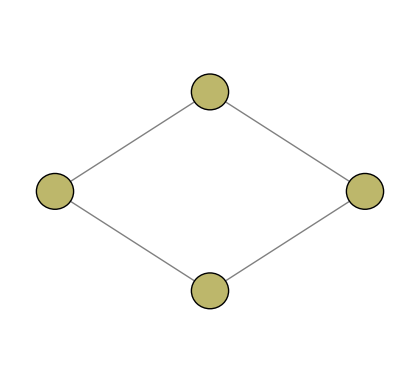
\includegraphics[scale=0.5]{Images/net_1_2_1.png}
\caption{}
\label{DiamondNet}
\end{figure}


To train the network, we generated an array of random 10000 points uniformly distributed in the interval $[0,1]$ and then computed the value of $f(x)$ for each random point. This gave us a data set to train our network on. A second data set was generated, in the same way, to be used for testing how well the network generalises. The network was trained using the stochastic gradient decent method for 50 epochs with a mini-batch size of 50. The evolution of the networks output as function of $x$ is shown in Fig.\ref{training}

\begin{figure}
\begin{subfigure}{.32\textwidth}
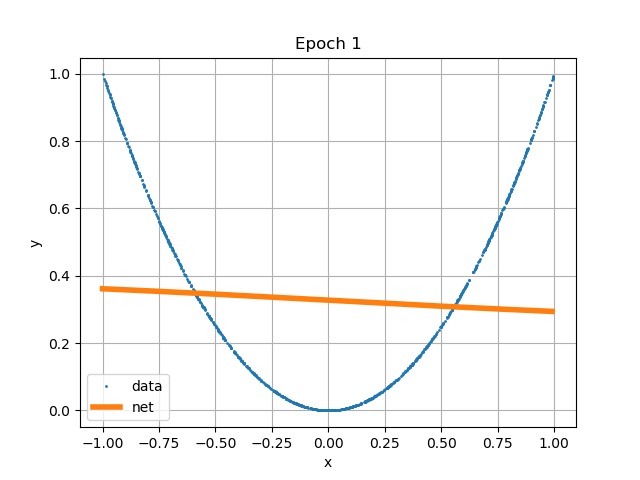
\includegraphics[scale=0.3]{Images/ALearningNet1.png}
\caption{}
\label{training1}
\end{subfigure}
\begin{subfigure}{.32\textwidth}
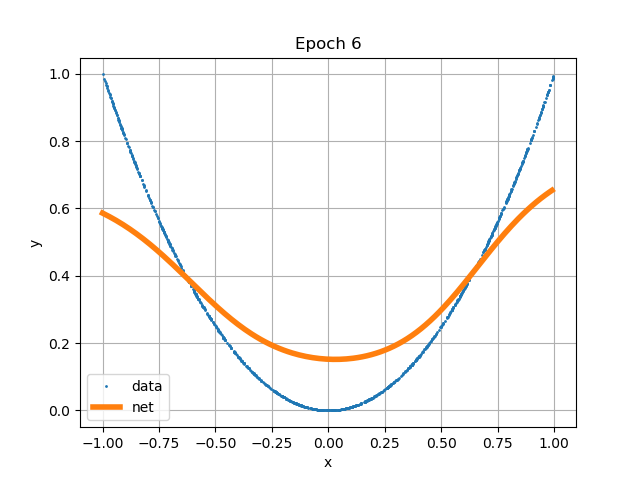
\includegraphics[scale=0.3]{Images/ALearningNet6.png}
\caption{}
\label{training2}
\end{subfigure}
\begin{subfigure}{.32\textwidth}
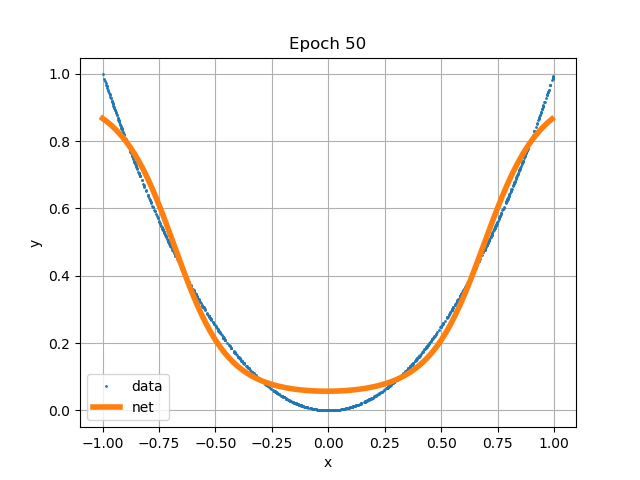
\includegraphics[scale=0.3]{Images/ALearningNet50.png}
\caption{}
\label{training3}
\end{subfigure}
\caption{}
\label{training}
\end{figure}

Once the network had been trained, we then looked at the performance of the network. The loss function used to evaluate the performance of the net was the squared Euclidean distance between the output of the net and the target output averaged over the test data.

The change in loss due to a variation in each of the networks parameters was calculated. We number the parameters of the network 0 to 6. The weights connecting the first two layers are numbers 0 and 1 while the weights connecting the second and third layers are numbered 2 and 3. The biases of the hidden layers are numbered 4 and 5 while the bias for the output neuron is given the number 6. Given the trained weights and biases $\{\omega_i\}$, we vary a particular parameter by adding a constant $\delta \omega_i$ ranging from -10 to 10 while holding all other parameters fixed. The results are shown in Fig.\ref{LossNearTrainedWeights}. We see each curve having a local minimum at $\delta\omega_i = 0$ indicating the network found a local minimum of the loss function while being trained.

\begin{figure}[H]
\center
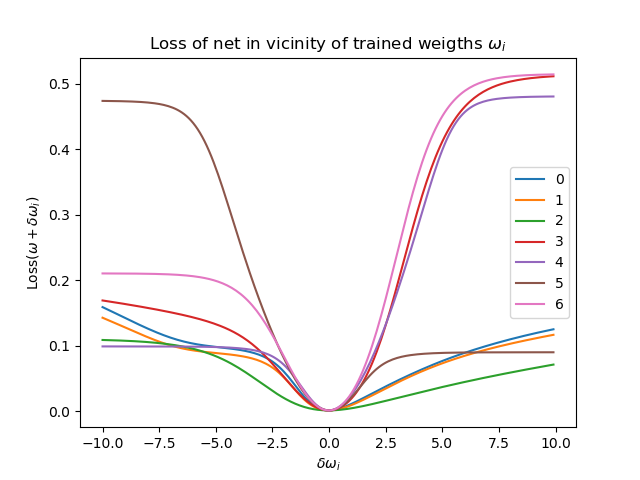
\includegraphics[scale=0.5]{Images/LossInVicinityOfTrainedWeights.png}
\caption{}
\label{LossNearTrainedWeights}
\end{figure}



\end{document}
